%https://arxiv.org/pdf/1611.03627.pdf
%https://www.sciencedirect.com/science/article/pii/S0168900219304991
%https://www.sciencedirect.com/science/article/pii/S0168900217305703

\chapter{\acrshort{IDEA} testbeam}
\label{chapter:ideatestbeam}

\epigraph{Ideas won't keep. Something \\ must be done about them.}{Alfred North Whitehead}

In this chapter, the usage of \acrshort{DQM4hep} outside of the \acrshort{AIDA}-2020 collaboration is discussed. This testbeam was the \acrfull{IDEA} combined testbeam. This was a complex testbeam environment, using five separate detector prototypes on the same testbeam, operating as a `vertical slice' of the detector concept for a future lepton collider.

The \acrshort{IDEA} testbeam environment and the detectors present are described. Following this, the development of the file readers for all of the datatypes used by the data acquisition systems is described, paying attention to the different needs of the different types of files. Then the development of the analysis modules that took the read raw data and converted it into monitor elements and human-readable plots is discussed. For this testbeam, the aim was first to recreate the existing monitoring solutions, but using the simpler and more systemic approach of \acrshort{DQM4hep} to combine them all on one machine and in one program. 

Following this, later work in using \acrshort{DQM4hep}'s analysis modules as a form of online data processing is described. Again, the usage of this aimed to recreate existing offline analysis that was done using ROOT. This was shown to be possible, and to be computationally lightweight enough to be done online during a testbeam.

\section{Introduction}
While \acrshort{DQM4hep} was intended from the beginning as a generic tool, it was developed largely within the \acrshort{AIDA}-2020 collaboration, which also promoted a variety of standards and guidelines for data acquisition devices, data formats, etc. In addition to this, it was also only tested on calorimeter-type detectors within the \acrshort{CALICE} collaboration. To be sure that \acrshort{DQM4hep} was truly generic -- capable of adapting to \textit{any} detector -- it was necessary to test it on a wider variety of detectors outside of the \acrshort{AIDA}-2020 and \acrshort{CALICE} collaborations.

An ideal opportunity arose for this in the form of the \acrshort{IDEA} testbeam. The \acrshort{IDEA} concept is a proposal for a detector for future lepton colliders such as the \acrshort{FCC}-ee or \acrshort{CEPC}, using a combination of a silicon vertex detector, large volume drift wire chamber with silicon micro-strips for tracking, a dual-readout calorimeter, and muon chambers. All of these subdetectors are contained within a low-mass superconducting solenoid and an iron flux return yoke. See Fig. \ref{figure:idea/detector-concept}.

\begin{figure}[h]
	\centering
	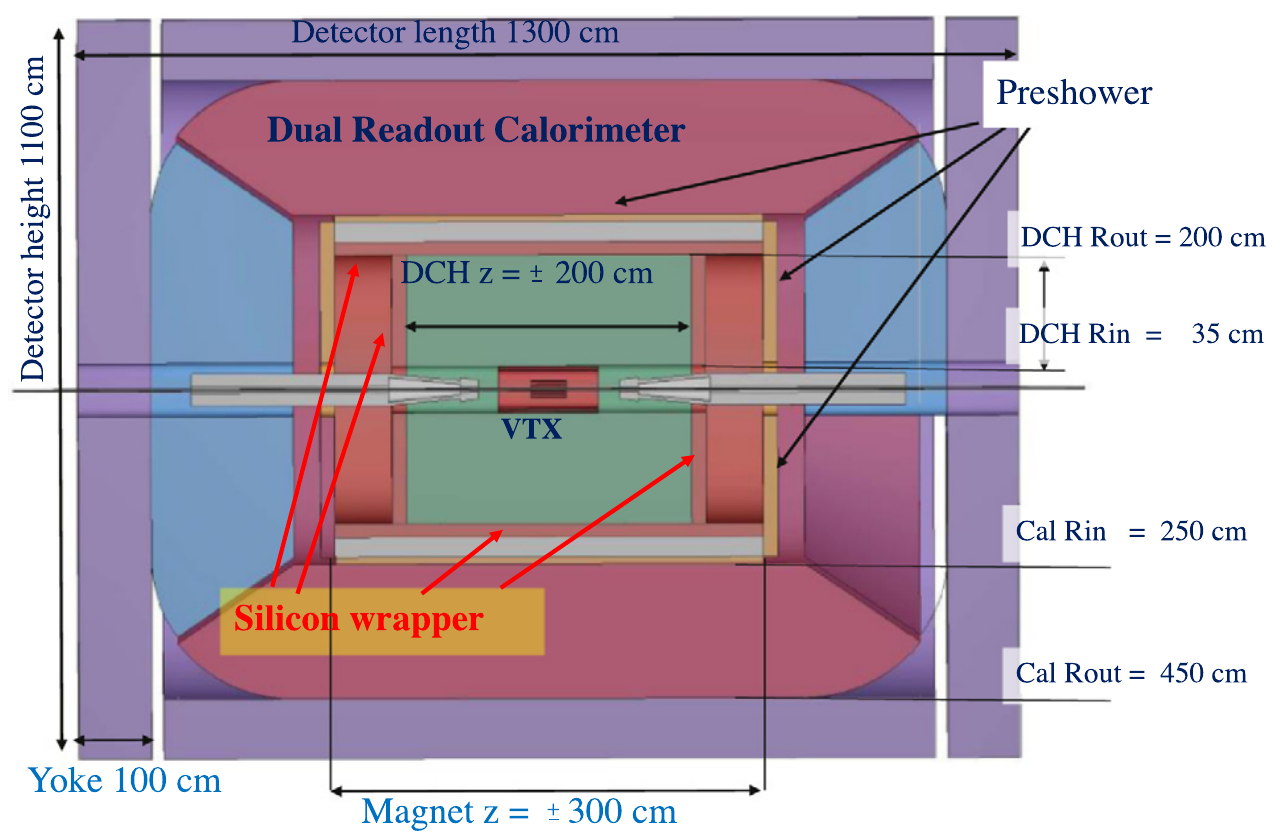
\includegraphics[width=0.65\textwidth]{../Pictures/IDEA/IDEA-concept.png}
	\caption{Schematic layout of the proposed \acrshort{IDEA} detector concept.}
	\label{figure:idea/detector-concept}
\end{figure}

The \acrshort{IDEA} testbeam was to take place in the H8 beamline area at the \acrshort{CERN} \acrshort{SPS}, including five separate prototypes, each representative of one subdetector of the \acrshort{IDEA} detector concept. This testbeam formed a `vertical slice' of the detector, operating each of the components in one testbeam to test not only each individual component, but how they interacted and could be used together to generate richer information about the beam.

\acrshort{DQM4hep} was offered as a possible unified monitoring solution that could integrate information from all of the detectors into a single tool. This provided convenience for the teams operating the testbeam and detectors, and an extremely valuable opportunity to test \acrshort{DQM4hep} out of its established operating range, using a wide variety of different detectors. The testbeam took place from the 5\textsuperscript{th}-12\textsuperscript{th} September, with a preparation period of one week before this for installation, setup and calibration.

\begin{figure}[hp]
	\centering
	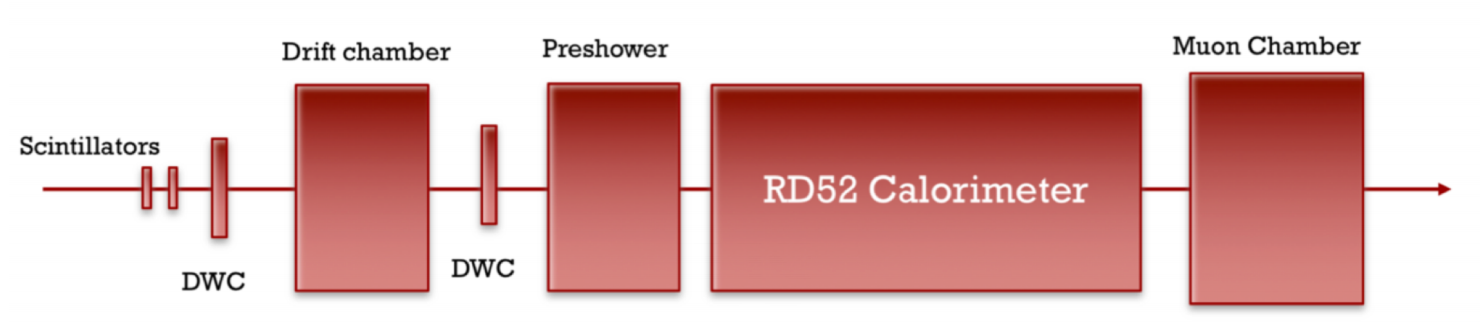
\includegraphics[width=0.65\textwidth]{../Pictures/IDEA/IDEA-testbeam-setup.png}
	\caption{Schematic of the position of the different detectors in the \acrshort{IDEA} combined testbeam.}
	\label{figure:idea/testbeam-layout}
\end{figure}

\begin{figure}[hp]
	\centering
	\includegraphics[width=0.65\textwidth]{../Pictures/IDEA/testbeam-area.jpg}
	\caption{Photograph of the testbeam area, looking east across the North Area of the \acrshort{CERN} \acrshort{SPS} facility.}
	\label{figure:idea/testbeam-photo}
\end{figure}

\section{Detector components}

\subsection{RD52 dual-readout calorimeter} % Another reference: https://arxiv.org/pdf/1703.09120.pdf
The \acrfull{DREAM} calorimeter, also called the RD52 calorimeter, is a dual-readout calorimeter built, developed and tested by the RD52 collaboration by researchers based in universities at Gagliari, Cosenza, Pavia, Pisa, Rome, Iowa State and Texas Tech. 

The aim of the calorimeter is to use both the \v{C}erenkov and scintillator techniques simultaneously (hence ``dual-readout'') to improve calorimetry, especially using calorimeters to measure four-vectors of jets and single hadrons, which suffer a reduced precision compared to electrons and photons. By comparing signals from \v{C}erenkov light and scintillator light, the electromagnetic shower fraction can be measured on an event-by-event basis, eliminating the effects of fluctuations. %Reference here: https://iopscience.iop.org/article/10.1088/1742-6596/404/1/012068/pdf

% Nigel: So far, all discussion of jets (themselves not described to date - evolution from quarks to collection of final state hadrons) has been around PFA, but this is not a PFA-based detector, perhaps helpful to add short discussion of this?

The prototype of the calorimeter used in the testbeam consists of 9 lead modules, each 9.3 $\times$ 9.3 $\times$ 250 cm\textsuperscript{3} in size, with a sampling fraction of 9\% and using a photomultiplier tube readout. From simulation studies, the hadronic energy resolution is expected to be approximately 30\%$/\sqrt{E}$ \cite{idea-dual-readout} \cite{idea-rd52}.

\subsection{Preshower}
The preshower uses two triple-GEM detectors with a surface area of 10 $\times$ 10 cm\textsuperscript{2}, using a strip readout with a 650 \textmu m pitch. The preshower also has a lead absorber layer of variable thickness, using a fixed layer of 5 mm plus additional interchangeable layers. The layers allow the absorber thickness to be varied between 1 and 2.5 $X_O$. The gas mixture used during the testbeam was Ar/CO\textsubscript{2}/CF\textsubscript{4}, and the efficiency expected from previous tests was 97\%. The spatial resolution is on the order of 100 \textmu m \cite{idea-gem}.

\subsection{Muon chamber}
The muon chamber comprises one triple-GEM detector (similar to the preshower) with an additional two \acrshort{muRWELL} prototypes of size 10 $\times$ 10 cm\textsuperscript{2}. The \acrshort{muRWELL} detectors have a spatial resolution of 40 \textmu m, and a rate capability of 10 MHz/cm\textsuperscript{2} \cite{idea-micro-rwell}.

\subsection{Drift chamber}
The prototype of the drift chamber used for the testbeam consisted of 12 layers, each with 12 drift cells of size 1$\times$1 cm\textsuperscript{2}, giving a total of 144 channels. According to a study of a similar detector prototype, this should give it a resolution of 100 \textmu m in the x- and y-plane, and 1 mm in the z-plane \cite{idea-drift-chamber} .

\subsection{Ancillary detectors}
The ancillary detectors are used to provide information about the position of the beam, the leakage of particles and showers from the detector volumes, and particle identification. They consist of two \acrlong{DWC}s (\acrshort{DWC}) in front of and behind the drift chamber; leakage counters surrounding the calorimeter; and a preshower detector and muon counter.

\section{Monitoring}
Existing monitoring within the collaboration was capable of producing histograms from the raw file formats, predominantly using C++ code directly to produce ROOT objects. Initially, the goal of the testbeam was to make the same plots used for the existing monitoring systems within \acrshort{DQM4hep}. The advantage of this would be that all of the plots were available in one place, making investigating any correlations between them easier.

The necessary components within \acrshort{DQM4hep} for monitoring were the creation of file readers for each device to make the data available to \acrshort{DQM4hep}, and analysis modules to use this data to create monitor elements.

\subsection{File readers}
Writing file readers for the different detectors meant first understanding the structure of their data and file types. Once data has arrived from the data acquisition device, each of the detectors wrote to a different `raw' format. However, the RD52 calorimeter, drift chamber, and muon and preshower all produced ROOT ntuple files as part of their data acquisition process, in addition to different file formats. It was decided to use these ROOT ntuples as the file format to read into \acrshort{DQM4hep}, as due to support for ROOT within the framework, reading data from ROOT ntuples is simpler.

For each of these three instruments a file reader was developed that walked through the ROOT trees, extracting data from the leaves event-by-event, then converted it to \acrshort{DQM4hep}'s inbuilt \texttt{GenericEvent} format. Choosing to make them into GenericEvents meant that there was no need to implement an additional event type, simplifying the connection between the file readers and analysis modules. The GenericEvent type was also easily suited to the type of data, as the majority of the data were series of numbers, which were easily converted into C++ vectors to store in the GenericEvent.

An additional motivation for using the ROOT ntuple as the data source was that some of the file types, notably the drift chamber, had not finalised their data structure at the beginning of the testbeam. Using the higher-level structure provided by a ROOT file would be easier to change in the future than reading in data in a binary, hex, text or \acrshort{CSV} format.

For the silicon photomultiplier \acrshort{GEM} data, the ``raw'' data format was a text file, containing an \acrshort{XML} header followed by a large amount of data in \acrfull{CSV}. This file could be loaded directly into \acrshort{DQM4hep}, the \acrshort{XML} header separated and parsed with \acrshort{DQM4hep}'s internal \acrshort{XML} parsing libraries, and the remaining data parsed. The comma-separated values could be easily parsed using the \texttt{dqm4hep::core::tokenize} function, which takes a string, a delimiter, and a vector, and parses the string into values separated by the delimiter, loading them into the vector. This made extracting the \acrshort{GEM} data extremely simple, even in this format. It also allowed the parameters in the \acrshort{XML} header, which included run numbers and physical information of the detector, to be passed into DQM4hep and the analysis module, using the \texttt{core::Run} object type.

\subsection{Analysis modules}
During the course of the testbeam, four analysis modules were developed, one for each detector. To begin with, these were `dummy' modules -- analysis modules that receive events then do nothing. Dummy modules like this are required to run file readers offline, but are simple to create as they can be produced from a template with minimal changes.

Once the file reader for the RD52 calorimeter was complete, the dummy analysis module for this detector was then changed into a functional module, \texttt{RD52MainModule}, to produce plots from the data. The RD52 was chosen as it was the most data-rich of the detectors in the testbeam, and also contained the ancillary detectors, which allow particle selection efficiencies to be studied.

During the course of the testbeam, the \texttt{RD52MainModule} was developed to read in and arrange data from the ROOT ntuples and arrange them into distinct vectors for the \acrshort{ADC}s, \acrshort{TDC}s, pedestals, and ancillaries. Following this, pedestal subtraction of all \acrshort{ADC} and \acrshort{TDC} channels was completed. Then the malfunctioning tiles and electronics that meant data had to be re-routed through other available channels was integrated so that the \acrshort{ADC} information in the analysis module represented the full state of the detector was completed. 

There was insufficient time at the testbeam to develop more complex monitoring than this, but development continued offline with saved data from the testbeam to continue the proof-of-concept. This will be discussed in more detail in the following section.

\section{Results}
Monitoring within \acrshort{DQM4hep} was able to replicate all the existing monitoring solutions, combining the monitoring tools for all four detector systems into one framework, with the exception of the drift chamber whose data type was not set during the testbeam, so file readers could not be implemented in time. 

Due to time constraints, more complex monitoring such as online processing was not implemented during the testbeam. However, following the testbeam it was decided that \acrshort{DQM4hep} could be used to perform some offline analysis functions in addition to the work at the testbeam, as a further proof of its ability to do this at testbeams. In this case, it performs in a similar role to ROOT, with the exception that it uses the existing analysis module infrastructure rather than scripts written specifically for ROOT, and can be run as soon as data is available for monitoring.

The analysis goals outlined to attempt to implement in \acrshort{DQM4hep} were performing the \acrshort{ADC} to energy calibration and the tower \acrshort{ADC} equalisation.

\subsection{ADC to energy calibration}

% Support for the response being linear
% No need for specific run number
% Nigel: This is an assertion but you need to give a little more information to support it, e.g. the fraction of non-electron particles in the beam is less than xx%, as from Cherenkov counters or other beam instrumentation or previous studies.

An important result for calibrating the RD52 detectors was to calibrate the \acrshort{ADC} response of the detector to the actual energy of the incident beam. It was known from prior testbeams that the \acrshort{ADC} response of the calorimeter was linear. Therefore, the calibration from \acrshort{ADC} to deposited energy can be extrapolated from a single run. This was done using Run 12659, a run using a 20 GeV electron beam incident on Tower 15, the centre of the calorimeter. The nature of the \acrshort{CERN} \acrshort{SPS} beamline means that electron beams are extremely pure, meaning that this run presents the most well-defined beam, making it ideal for energy calibration. This also means that particle selection to exclude other particles is not necessary.

To calibrate for energy, the total \acrshort{ADC} for each event was found by summing the individual \acrshort{ADC} of each channel in the event after the pedestal subtraction. This produced a spectrum of the total \acrshort{ADC} count for all channels (Fig. \ref{figure:testbeam/results/total-adc-20}).

The data was then fitted with a gaussian using ROOT to determine the mean and standard deviation, and the value of the mean \acrshort{ADC} taken to be the \acrshort{ADC} value for a 20 GeV event. This means that for a 20 GeV event, the total \acrshort{ADC} count will be 296.3 $\pm$ 0.9. The energy of any given ADC can then be found using:

\begin{equation}
	E_{GeV} = \frac{E_{ADC}}{14.815}
\label{eq:adc-to-energy}
\end{equation}

where $E_{GeV}$ is the energy in GeV, and $E_{ADC}$ is the energy in terms of ADC.

This can then be checked by examining Run 12512, which is an 80 GeV run using a secondary beam of predominantly pions, with some muons. According to Equation \ref{eq:adc-to-energy}, an energy of 80 GeV should translate to an ADC of 1185.2. The total ADC histogram for the 80 GeV run can be seen in Fig. \ref{figure:testbeam/results/total-adc-80}, showing that the mean is 1191, which corresponds to an energy of 92.94 GeV.

% Nigel: Sounds sensible, would you consider doing the same for all data and putting into a plot to illustrate this more systematically?

\begin{figure}[p]
	\centering
	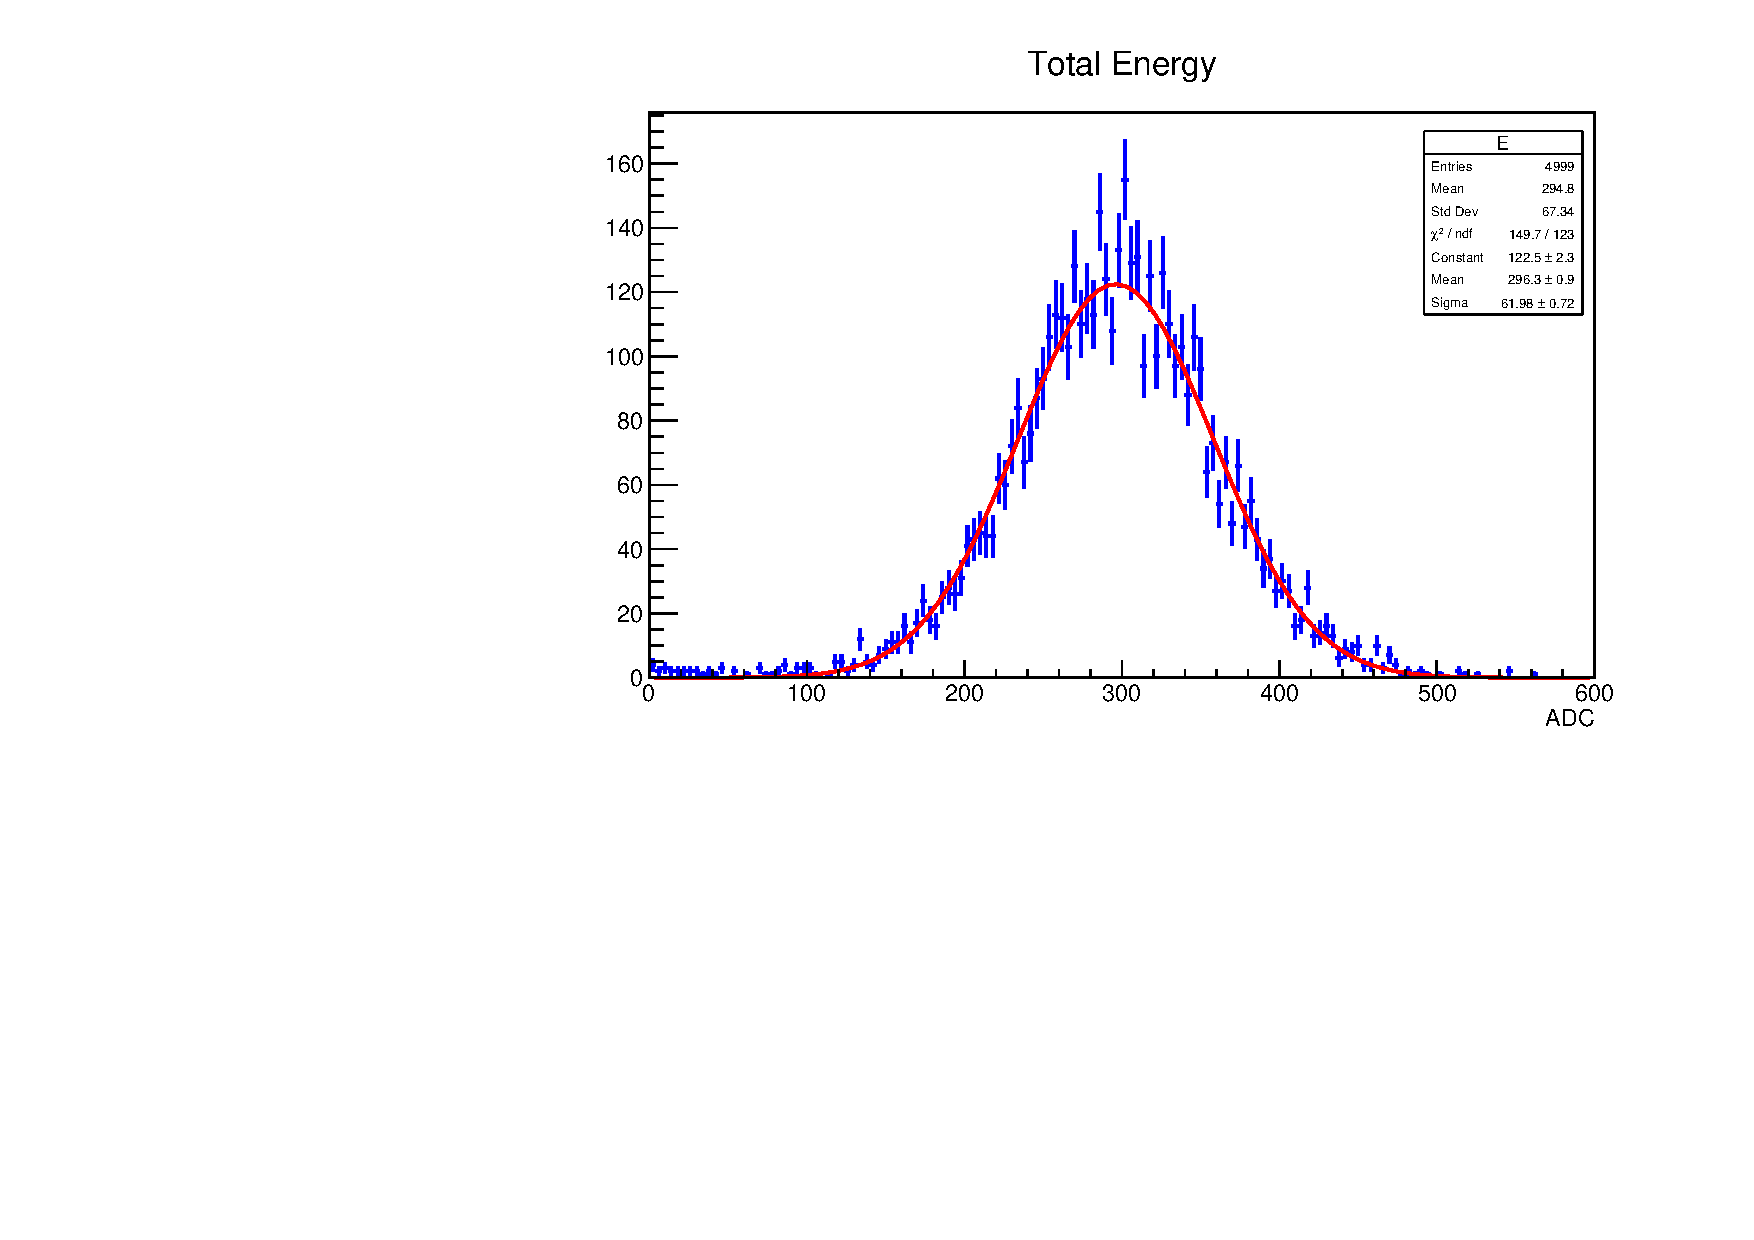
\includegraphics[width=0.95\textwidth]{../Pictures/IDEA/totalEnergyBoth.pdf}
	\caption{Histogram of total \acrshort{ADC} in the calorimeter in Run 12659 (20 GeV electrons, Tower 15).}
	\label{figure:testbeam/results/total-adc-20}
\end{figure}

\begin{figure}[p]
	\centering
	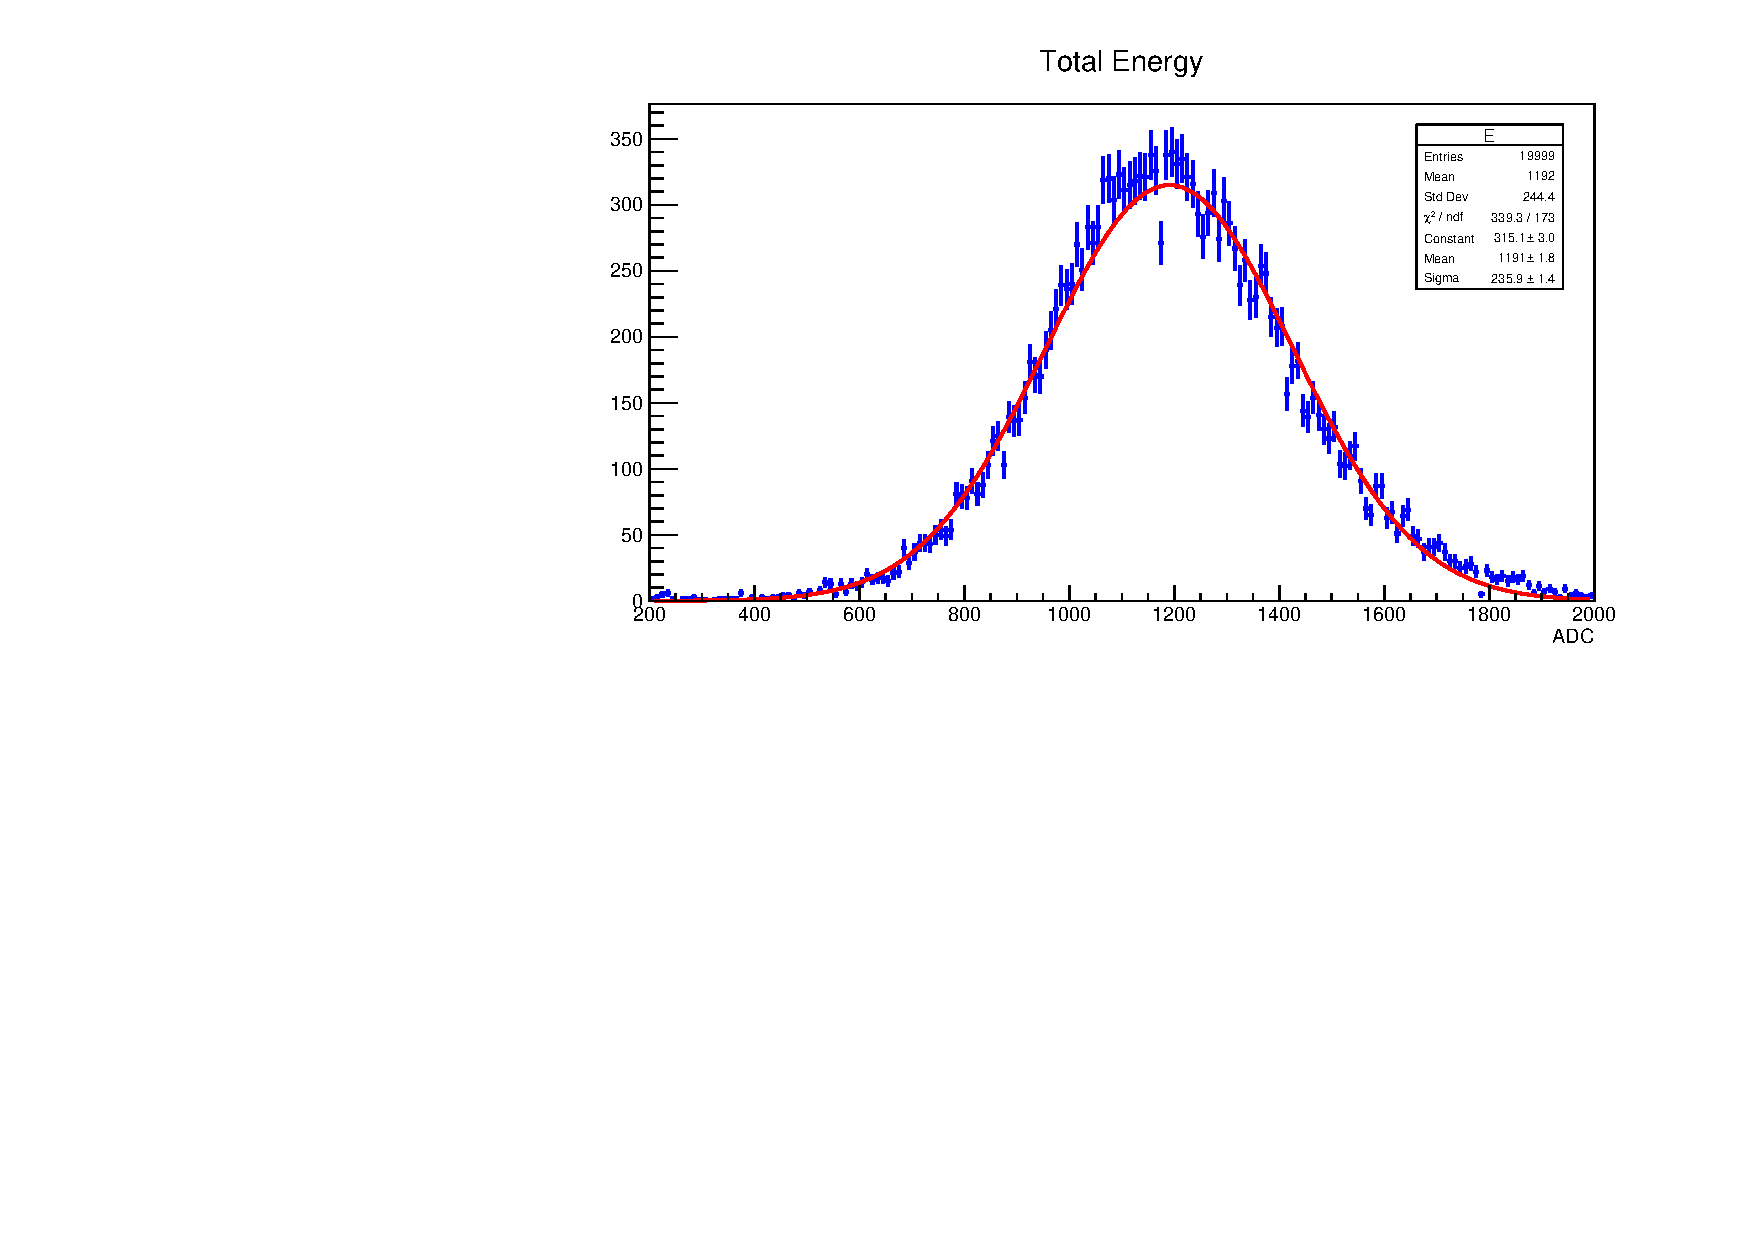
\includegraphics[width=0.95\textwidth]{../Pictures/IDEA/totalEnergy80GeV.pdf}
	\caption{Histogram of total \acrshort{ADC} in the calorimeter in Run 12512 (80 GeV pions and muons, Tower 15).}
	\label{figure:testbeam/results/total-adc-80}
\end{figure}

\subsection{Tower ADC calibration}
\label{section:tower-calibration}
Due to a large number of tasks for setting up the testbeam, performing a calibration of the high voltages of the individual towers was not possible in time, so the calorimeter \acrshort{ADC}s were not calibrated to have a uniform response. To account for this, calibration runs were taken, where the beam was incident on each individual tower for the whole run, repeated for each tower in the calorimeter. These runs allow the calibration to be done after the testbeam with the data. The layout of the towers in the calorimeter for the testbeam can be seen in Fig. \ref{figure:testbeam/results/tower-layout}.

\begin{figure}[h]
	\centering
	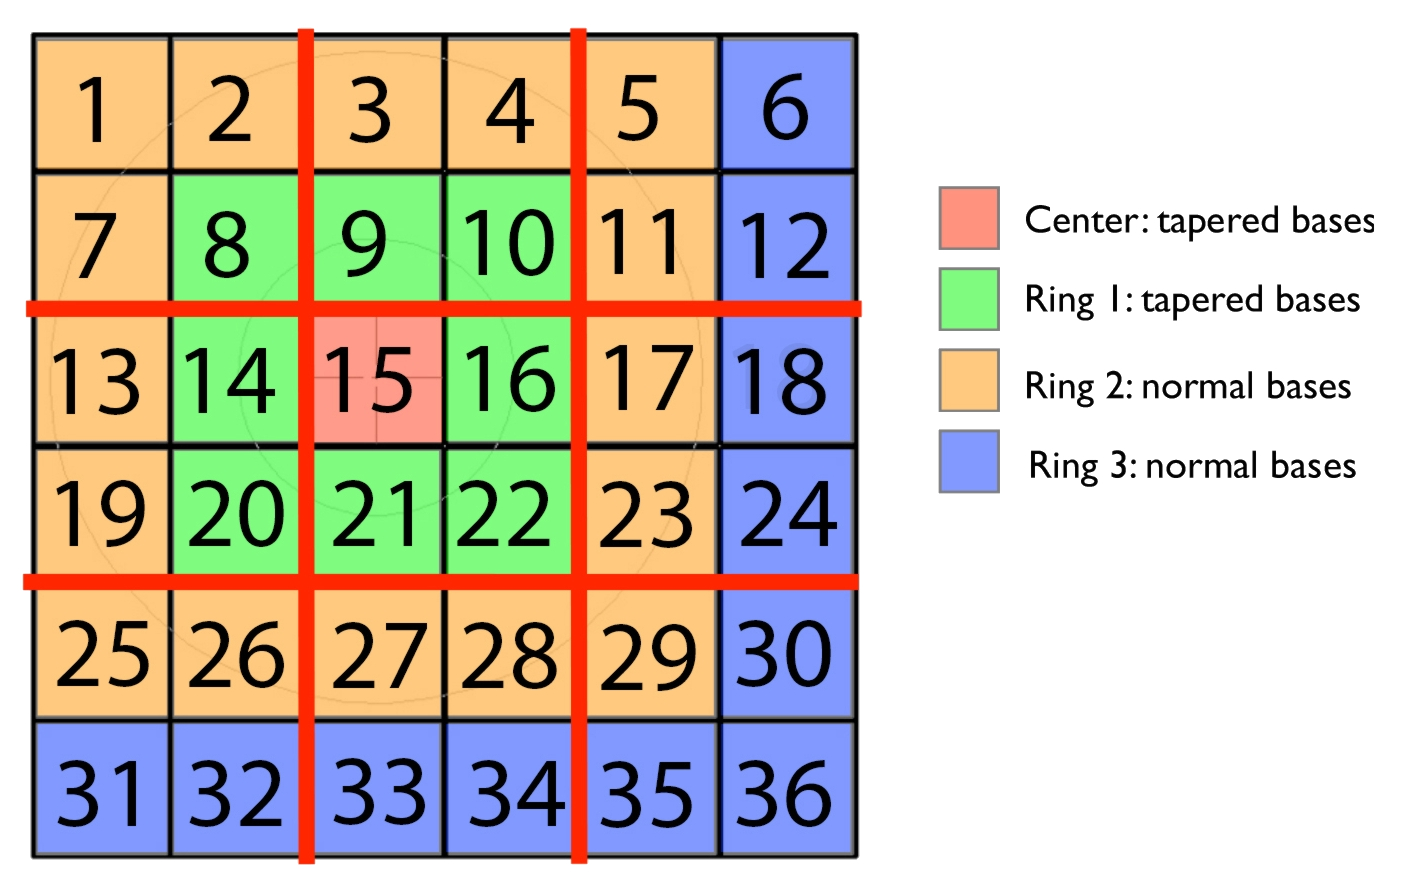
\includegraphics[width=0.75\textwidth]{../Pictures/IDEA/RD52-towers.jpg}
	\caption{The layout of the calorimeter modules (``towers'') in the layers of the RD52 calorimeter used in the \acrshort{IDEA} testbeam.}
	\label{figure:testbeam/results/tower-layout}
\end{figure}

Two sets of calibration runs were performed. The first set covered Towers 1-29 with an 80 GeV secondary beam (primarily pions with some muons)\footnote{Due to the nature of the \acrshort{SPS} testbeam facility, the composition of secondary beams is not well-defined. Normally it is determined using detectors in the beamline.}. The second set used a 20 GeV pure electon beam, covering Towers 30-36 plus Tower 15. Tower 15 received runs in both sets in order to calibrate the two sets to each other. The run numbers corresponding to each tower is given in Table \ref{table:idea/calibrationruns}.

\begin{table}[h]
\centering
	\begin{tabular}{ c c | c c }
	\hline \hline
	\textbf{Tower} & \textbf{Run No.} & \textbf{Tower} & \textbf{Run No.} \\ \hline \hline
	 1 & 12545 & 16 & 12526 \\
	 2 & 12556 & 17 & 12567 \\
	 3 & 12558 & 18 & 12633 \\
	 4 & 12560 & 19 & 12591 \\
	 5 & 12601 & 20 & 12612 \\
	 6 & 12638 & 21 & 12530 \\
	 7 & 12598 & 22 & 12528 \\
	 8 & 12514 & 23 & 12569 \\
	 9 & 12518 & 24 & 12639 \\
	10 & 12521 & 25 & 12610 \\
	11 & 12600 & 26 & 12609 \\
	12 & 12636 & 27 & 12607 \\
	13 & 12539 & 28 & 12604 \\
	14 & 12628 & 29 & 12602 \\
	15 & 12512 &    &    \\ \hline
	\end{tabular}
	\caption{Table of the run numbers and corresponding tower numbers for the calibration runs.}
	\label{table:idea/calibrationruns}
\end{table}

% Add run duration, particle type, number of triggers, etc. and merge with Table 4.2

The initial approach to calibrate the towers was to make a histogram of the \acrshort{ADC}s of the scintillators of all events in the tower under the beamspot, for each of the 29 pion runs (see Fig. \ref{figure:testbeam/results/towerplot-raw-uncalibrated}). From these, a gaussian fit is used to determine the mean of each channel, shown in Fig. \ref{figure:testbeam/results/towerplot-mean-uncalibrated-all}. The calibration coefficient is then calculated: \\

% Nigel: How much/what data were taken, 1st we have heard of 29 runs so far? Merge two tables 4.1 and 4.2.

\begin{equation}
	C_i = \frac{\mu_{15}}{\mu_i}
\label{eq:calibration-coeff}
\end{equation}

where $C_i$ is the calibration coefficient for the i\textsuperscript{th} tower, $\mu_{15}$ is the mean \acrshort{ADC} for tower 15, $\mu_i$ is the mean \acrshort{ADC} of the i\textsuperscript{th} tower. Tower 15 was used as the reference.

The process needed to obtain the calibration coefficients was the use of a bash script that automated the generation of \acrshort{XML} steering files for the 29 runs and another bash script that automated the execution of the \acrshort{DQM4hep} analysis modules and merging the information into one file.

The analysis module was then re-run, multiplying all \acrshort{ADC} values by the calibration coefficient for each tower. The results of the calibration are shown in Figs. \ref{figure:testbeam/results/towerplot-raw-calibrated} and \ref{figure:testbeam/results/towerplot-mean-calibrated-all}. This did not result in a uniform calibration of all \acrshort{ADC}s. This is possibly due to the composition of the beam, as this calibration procedure was done without any particle selection.

% Nigel: Discuss this, and whether it is important if the beam content is constant in time when scanning different towers

Also, discuss how the beam purity can vary within the beam spot and what the beam energy spread is for electrons at 20 GeV vs. the pion beam at 80 GeV. 

A pattern of increasing mean \acrshort{ADC}s can be seen from Towers 14-19, which repeats in Towers 20-25. These align with the rows on the calorimeter, and this periodic pattern is is likely due to some form of leakage or other geometric effect in the calorimeter. 

\begin{figure}[hp]
	\centering
	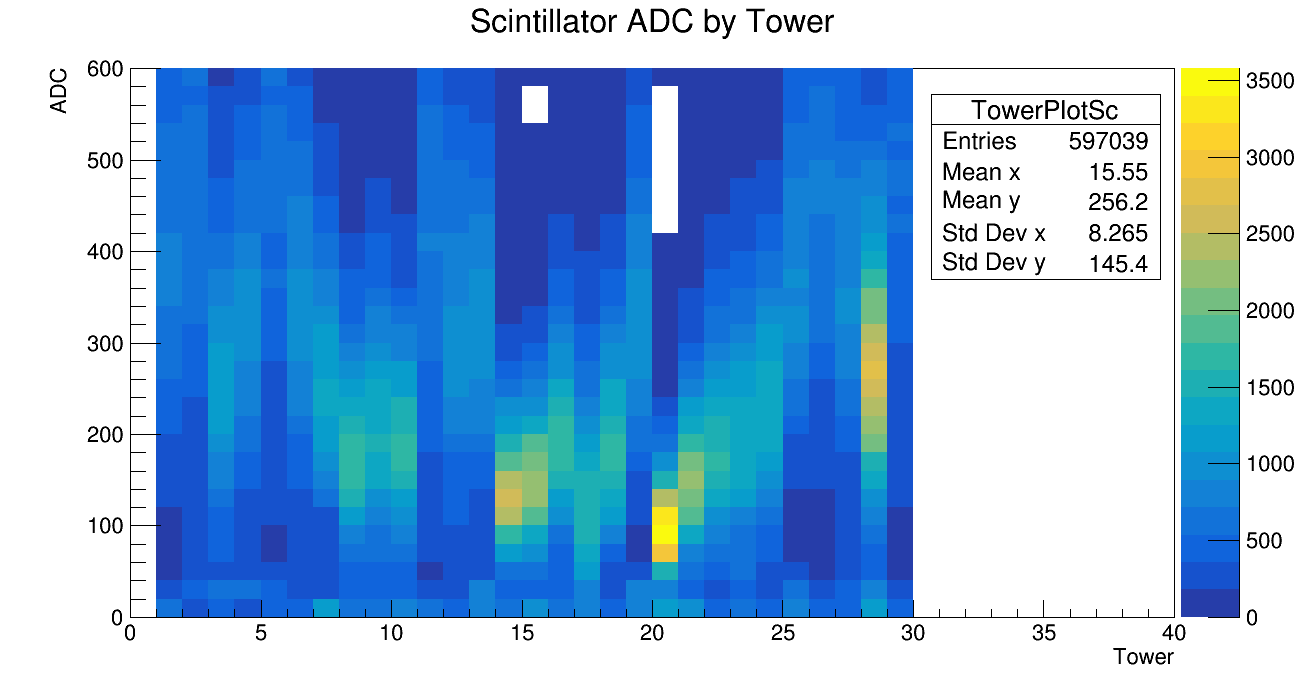
\includegraphics[width=0.95\textwidth]{../Pictures/IDEA/Calibration/new-towerplot-density-uncalibrated.png}
	\caption{Histogram of scintillator \acrshort{ADC}s for Towers 1-29 before calibration.}
	\label{figure:testbeam/results/towerplot-raw-uncalibrated}
\end{figure}

\begin{figure}[hp]
	\centering
	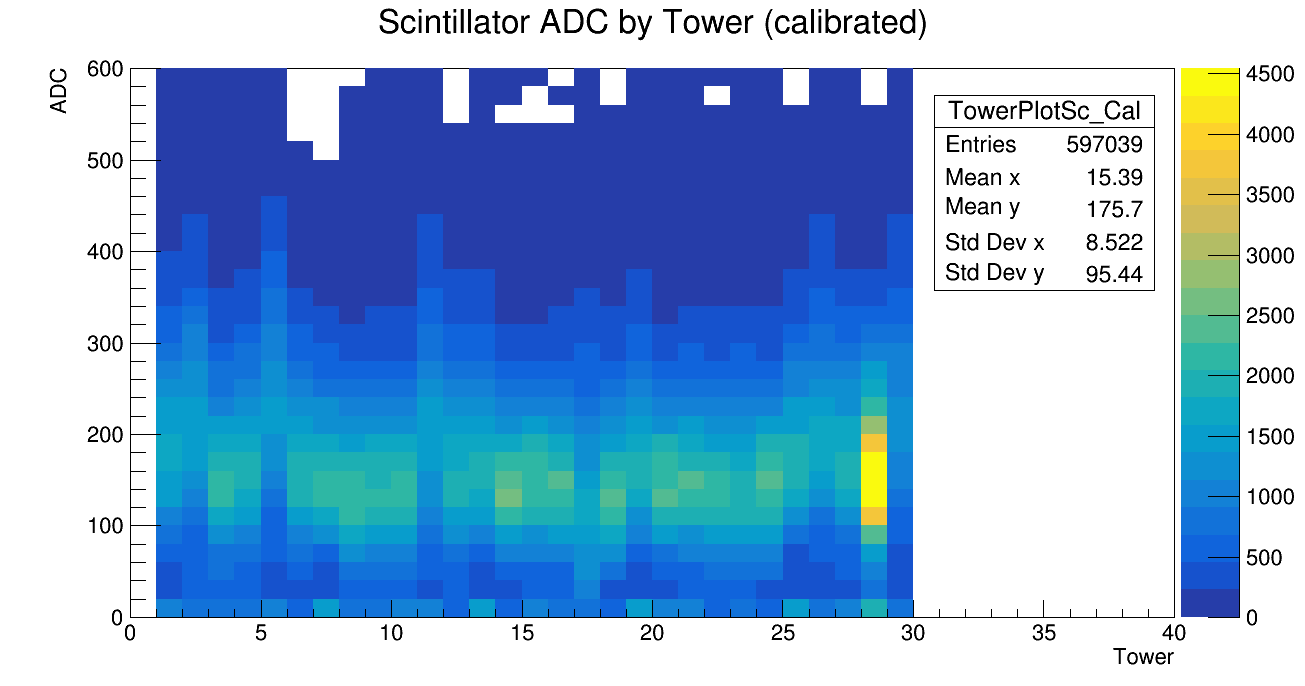
\includegraphics[width=0.95\textwidth]{../Pictures/IDEA/Calibration/new-towerplot-density-calibrated.png}
	\caption{Histogram of scintillator \acrshort{ADC}s for Towers 1-29 after applying the calibration using all particles.}
	\label{figure:testbeam/results/towerplot-raw-calibrated}
\end{figure}

\begin{figure}[hp]
	\centering
	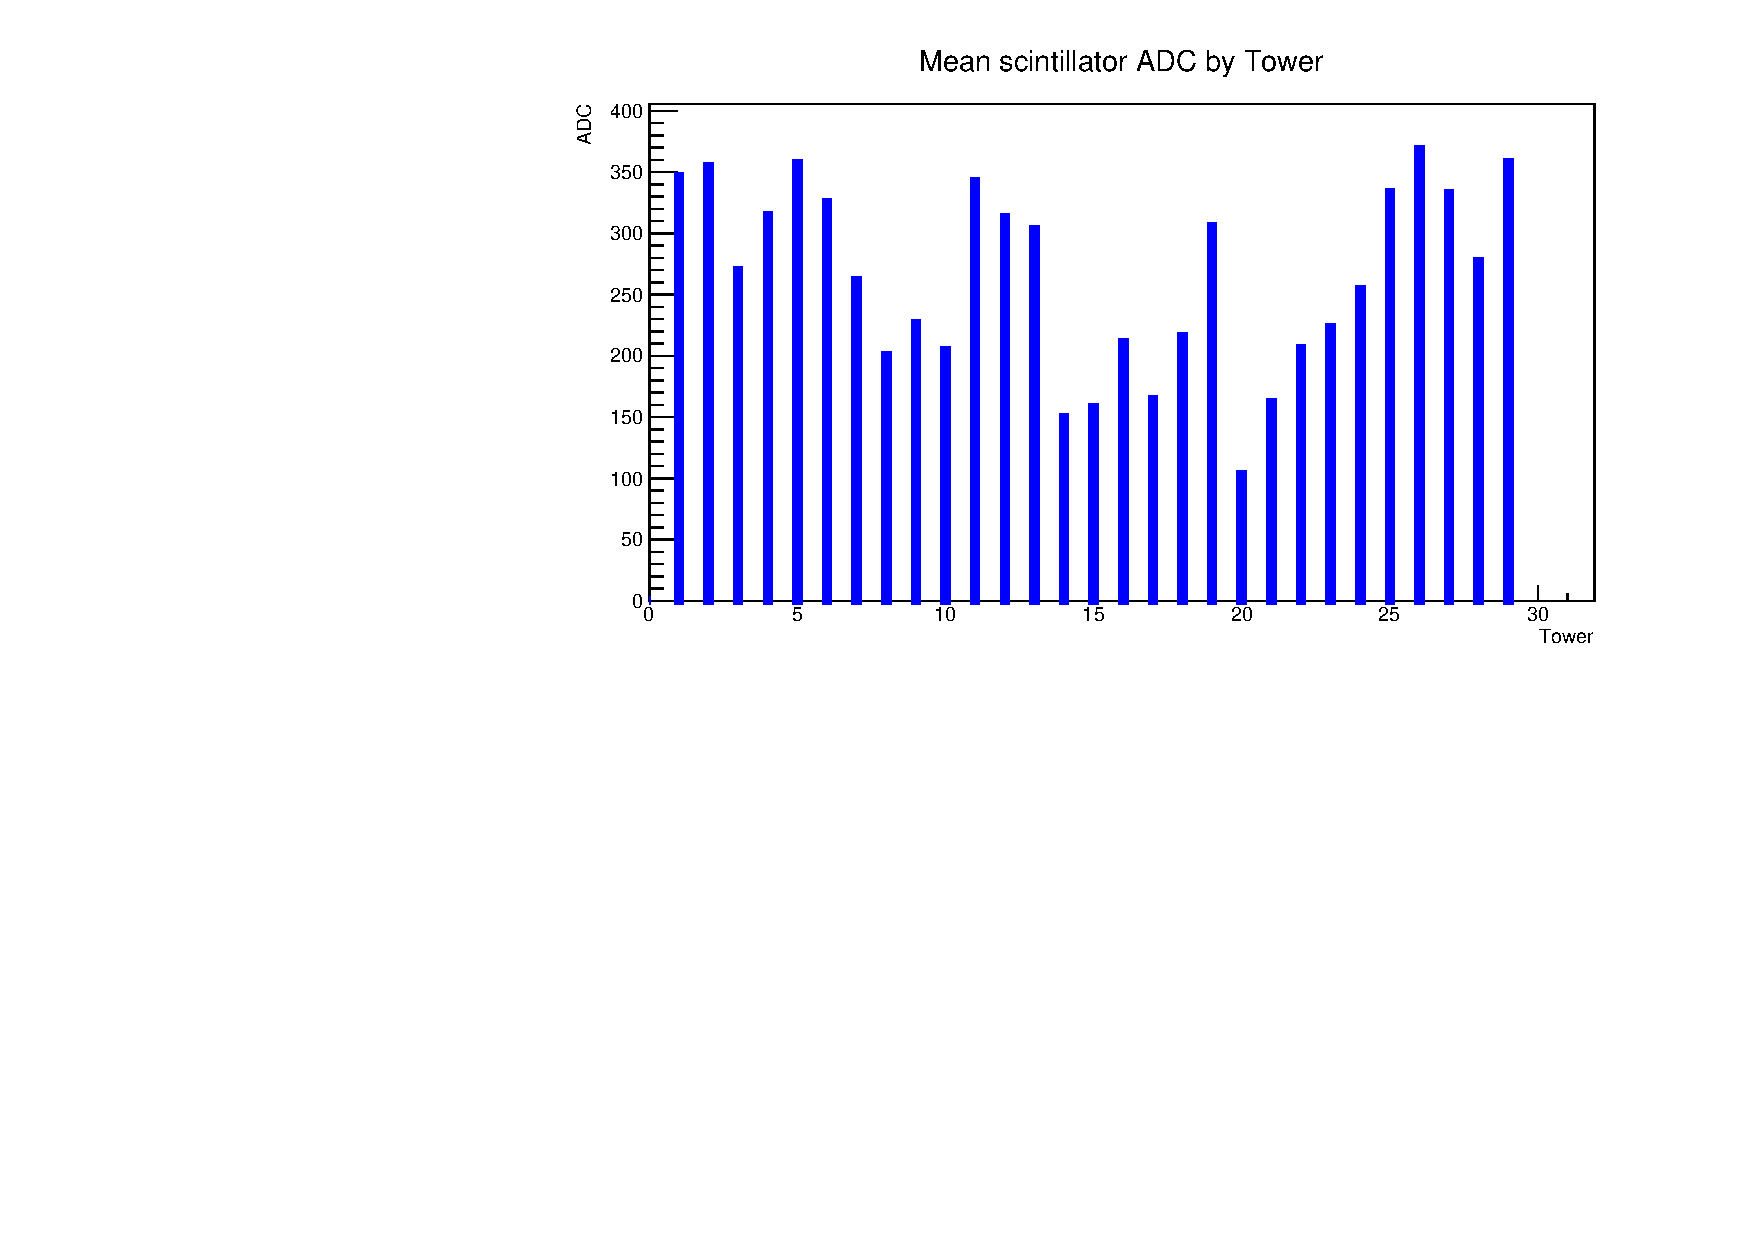
\includegraphics[width=0.95\textwidth]{../Pictures/IDEA/Calibration/new-towerplot-uncal.pdf}
	\caption{Histogram of mean scintillator \acrshort{ADC}s for Towers 1-29 before calibration.}
	\label{figure:testbeam/results/towerplot-mean-uncalibrated-all}
\end{figure}

\begin{figure}[hp]
	\centering
	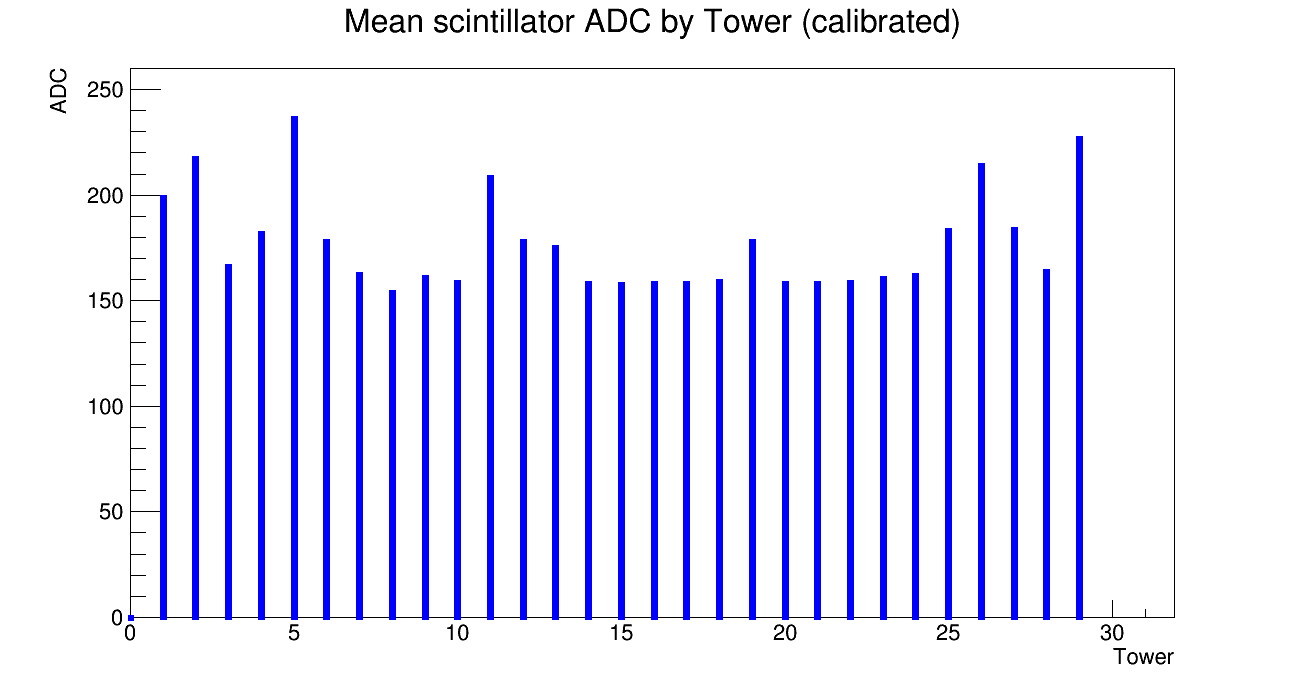
\includegraphics[width=0.95\textwidth]{../Pictures/IDEA/Calibration/new-towerplot-all-cal.png}
	\caption{Histogram of mean scintillator \acrshort{ADC}s for Towers 1-29 after applying the calibration using all particles.}
	\label{figure:testbeam/results/towerplot-mean-calibrated-all}
\end{figure}

Because particles were not selected, the calibration here does not account for the different ways pions and muons deposit energy in the calorimeter. Pions will produce hadronic showers, spreading their energy within a certain radius and depth dependent upon the pion's energy and the nuclear interaction length of the calorimeter. Muons instead act as minimum ionising particles (\acrshort{MIP}s), depositing energy along their path through the calorimeter via ionisation losses.

In order to address this, calibration was done twice more, using particle selection criteria determined by another member of the collaboration \cite{idea-particle-selection}.

\subsubsection{Calibration with muons}
Given that muons in the calorimeter will leave a \acrshort{MIP}-like signal, muons were chosen to be used for calibrating the calorimeter. Muons were selected using two cuts: 

\begin{itemize}
	\item ADC of the muon counter $>$ 10
	\item ADC of the preshower detector $<$ 20
\end{itemize}

The same procedure as in Section \ref{section:tower-calibration} was then used, using only muons. The average ADCs of all towers using muons before calibration can be seen in Fig. \ref{figure:testbeam/results/towerplot-mean-uncalibrated-muons}, showing that the response to muons is overall much more uniform across the calorimeter.

% Nigel: discuss further, response to muons looks surprisingly non-uniform; are you sure about the description of relative uniformity of muon response compared to pions? 4.11 vs. 4.9, probabl easier if ch. 17 was not so high?

The same calibration coefficients were then applied to all particles (Fig. \ref{figure:testbeam/results/towerplot-mean-muoncalibrated-all}) and pions only (\ref{figure:testbeam/results/towerplot-mean-muoncalibrated-all}). 

\begin{figure}[h]
	\centering
	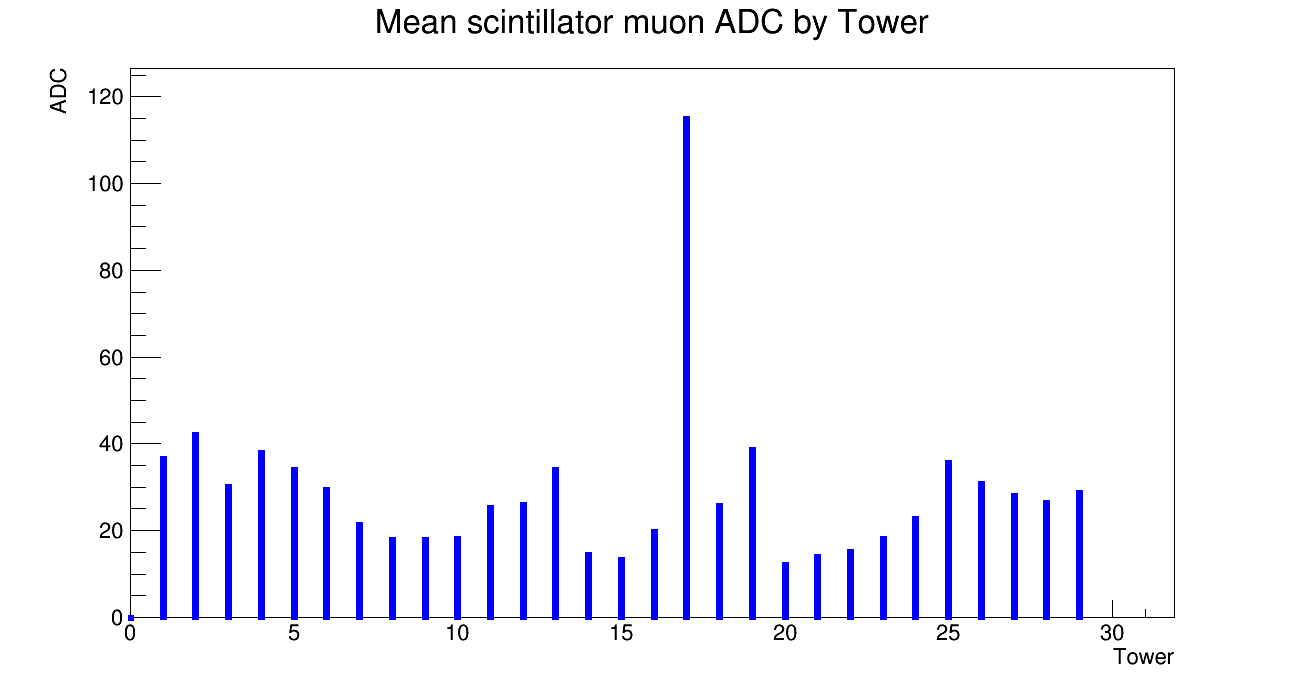
\includegraphics[width=0.95\textwidth]{../Pictures/IDEA/Calibration/new-towerplot-muon-uncal.png}
	\caption{Histogram of mean scintillator \acrshort{ADC}s for Towers 1-29 using only muons, before calibration.}
	\label{figure:testbeam/results/towerplot-mean-uncalibrated-muons}
\end{figure}

\begin{figure}[h]
	\centering
	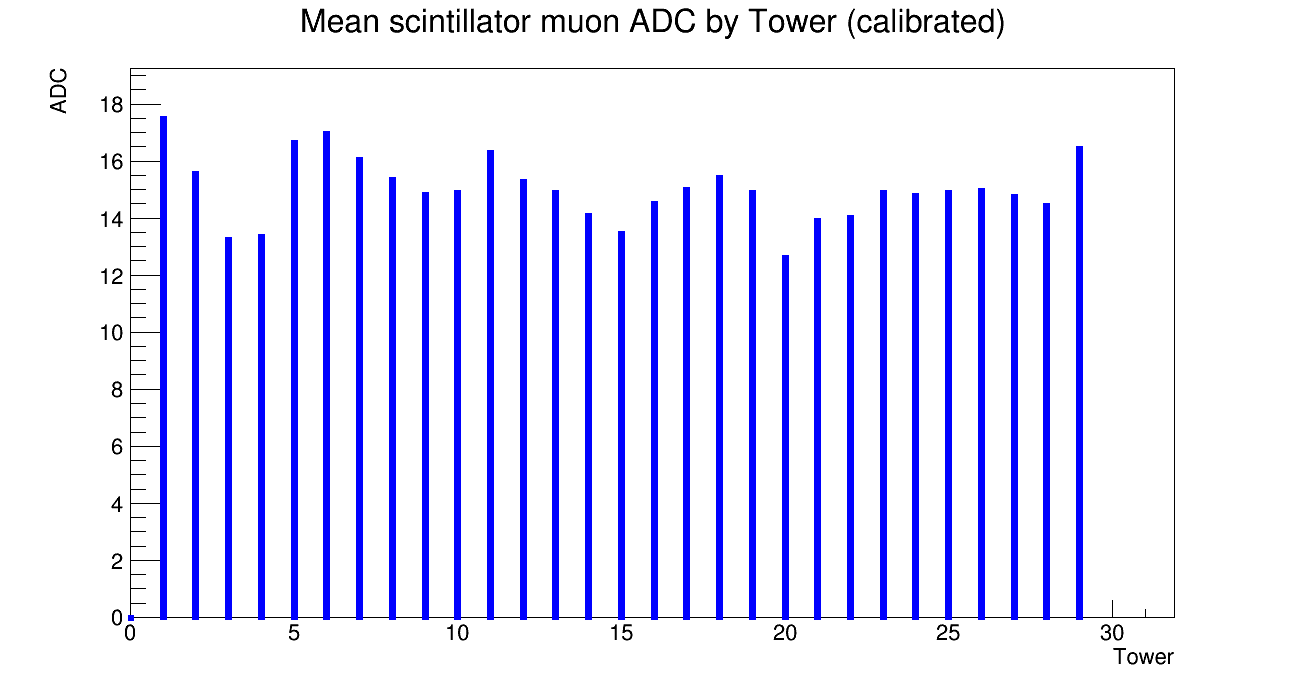
\includegraphics[width=0.95\textwidth]{../Pictures/IDEA/Calibration/towerplot-scintillator-mean-muoncalibrated-muons.png}
	\caption{Histogram of mean scintillator \acrshort{ADC}s for Towers 1-29 using only muons, after applying the calibration using only muons.}
	\label{figure:testbeam/results/towerplot-mean-muoncalibrated-muons}
\end{figure}

\begin{figure}[h]
	\centering
	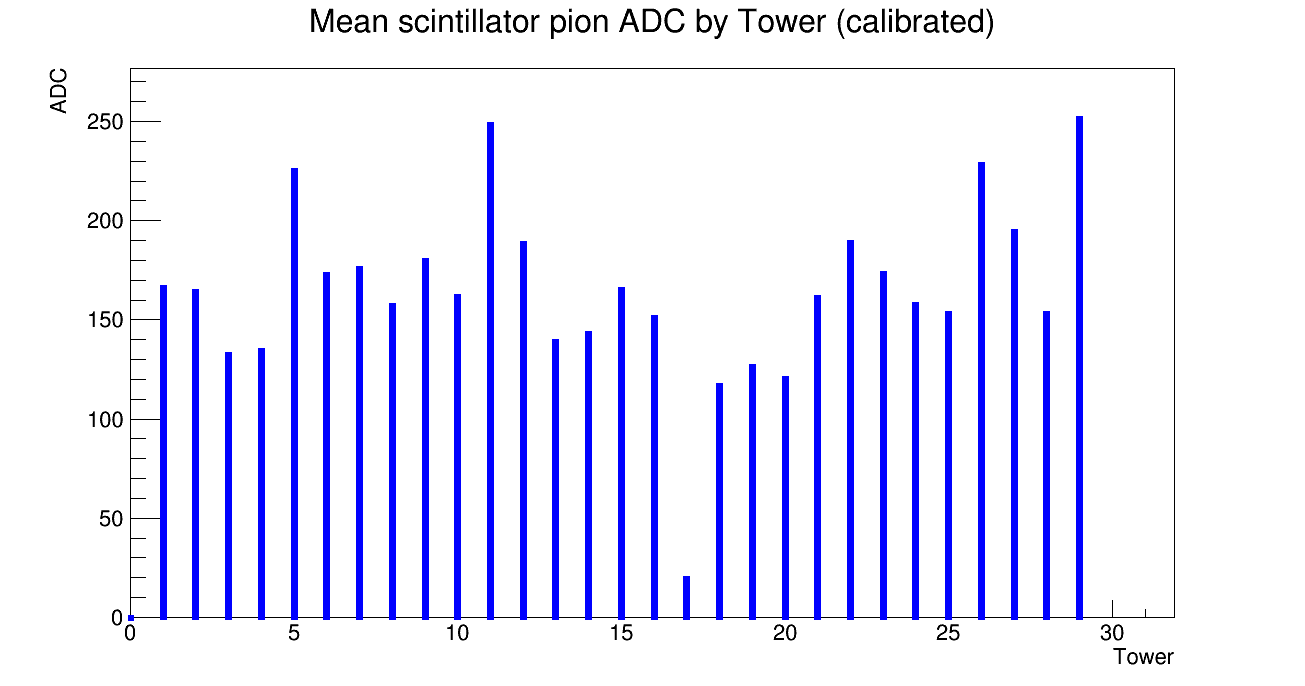
\includegraphics[width=0.95\textwidth]{../Pictures/IDEA/Calibration/towerplot-scintillator-mean-muoncalibrated-pions.png}
	\caption{Histogram of mean scintillator \acrshort{ADC}s for Towers 1-29 using only pions, after applying the calibration using only muons.}
	\label{figure:testbeam/results/towerplot-mean-muoncalibrated-pions}
\end{figure}

\begin{figure}[h]
	\centering
	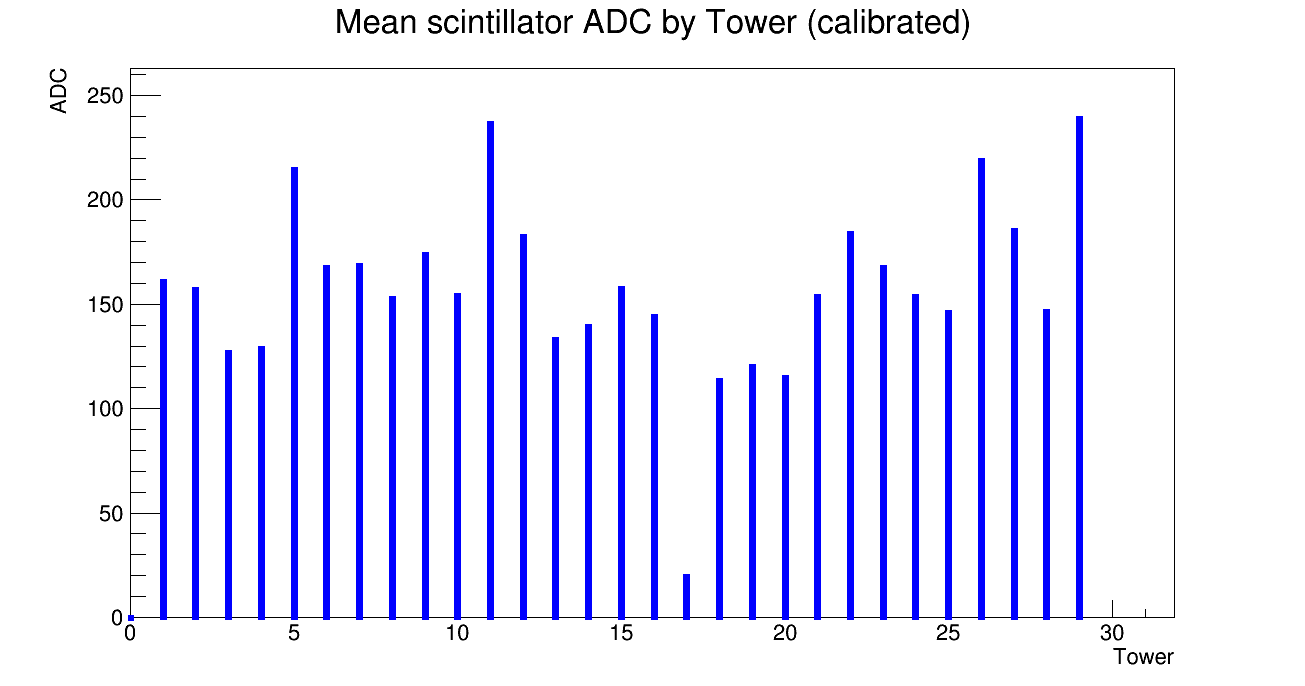
\includegraphics[width=0.95\textwidth]{../Pictures/IDEA/Calibration/towerplot-scintillator-mean-muoncalibrated-all.png}
	\caption{Histogram of mean scintillator \acrshort{ADC}s for Towers 1-29 using all particles, after applying the calibration using only muons.}
	\label{figure:testbeam/results/towerplot-mean-muoncalibrated-all}
\end{figure}

While the equalisation of pions using the muon response is not as uniform as that for equalising all towers using all particles, it does perform some equalisation, and removes the geometric pattern in the towers. It highlights that Tower 17 appears to have had an unusually high muon response, and as a result of the extremely low equalisation coefficient used to remedy this, produces very low \acrshort{ADC} responses in that Tower to other particles. This may be due to a technical fault with that tower, or some geometric effect.

% Nigel: does it make sense to use calibration like this on this channel? Please show the raw ADC distribution for all channels rather than just the mean, e.g. 6x6 plot of postage stamp sized images so illustrate that they are plausibly gassian in shape.

The usage of \acrshort{DQM4hep} to perform this calibration, similar to that completed by another member of the RD52 collaboration \cite{idea-equalisation} demonstrates that DQM4hep can be used not only for online monitoring and data quality monitoring, but also online or nearly-online analysis of testbeam data.

\begin{table}[hp]
\centering
	\begin{tabular}{ c c c c c}
	\hline \hline
	\textbf{Tower} & \textbf{Run No.} & $C_{all}$ & $C_{\pi}$ \\ \hline
	 1 & 12545 & 0.4551 & 0.3665 \\
	 2 & 12556 & 0.4450 & 0.3184 \\
	 3 & 12558 & 0.5842 & 0.4455 \\
	 4 & 12560 & 0.5008 & 0.3534 \\
	 5 & 12601 & 0.4417 & 0.3957 \\
	 6 & 12638 & 0.4845 & 0.4564 \\
	 7 & 12598 & 0.6026 & 0.6262 \\
	 8 & 12514 & 0.7617 & 0.7470 \\
	 9 & 12518 & 0.6953 & 0.7522 \\
	10 & 12521 & 0.7729 & 0.7400 \\
	11 & 12600 & 0.4607 & 0.5302 \\
	12 & 12636 & 0.5040 & 0.5172 \\
	13 & 12539 & 0.5203 & 0.3943 \\
	14 & 12628 & 1.0561 & 0.9303 \\
	15 & 12512 & 1.0000 & 1.0 \\
	16 & 12526 & 0.7488 & 0.6825 \\
	17 & 12567 & 0.9609 & 0.1170 \\
	18 & 12633 & 0.7315 & 0.5217 \\
	19 & 12591 & 0.5163 & 0.3486 \\
	20 & 12612 & 1.5273 & 1.1079 \\
	21 & 12530 & 0.9764 & 0.9527 \\
	22 & 12528 & 0.7652 & 0.8903 \\
	23 & 12569 & 0.7056 & 0.7376 \\
	24 & 12639 & 0.6210 & 0.5899 \\
	25 & 12610 & 0.4735 & 0.3769 \\
	26 & 12609 & 0.4278 & 0.4379 \\
	27 & 12607 & 0.4738 & 0.4778 \\
	28 & 12604 & 0.5690 & 0.5078 \\
	29 & 12602 & 0.4405 & 0.4671 \\ \hline \hline
	\end{tabular}
	\caption{Table of towers in the RD52 calorimeter with the run number of their calibration run, and calibration coefficients for all particles ($C_{all}$) and muons ($C_{\mu}$).}
	\label{table:idea/calibrationruns}
\end{table}

% Show these results in a plot

% Add a 6x6 'heat map' type plot, showing mean ADC value from the gassian fit as the z axis, and comment on the results, is there a pattern that could suggest it is related to leakage or the 'cone pattern' of the detectors (green square in Fig.)? 
% Related to this, recommend that you add this as a monitoring module, and use the fact that this was done quickly to illustrate how easily the DQM4hep architecture allows such an addition to be made.  This would be a good way to end the chapter too.